\section{Finite Sum Optimization}
\Title{Variance Reduction Technique}
We try to reduce the variance $\sigma^2$ in order to improve the bound of SGD:
\textbf{Mini-batch sampling}: use a small batch of samples instead of one to estimate the gradient at every iteration: replace $\nabla f(\xx_t, \xxi_t)$ with $\frac{1}{b} \sum_{i=1}^b{\nabla f(\xx_t, \xxi_{t, i})}$. The variance will be $\BigO(b)$ times smaller. \\
\textbf{Importance sampling}: Instead of sampling from $\xxi \sim P$ , we can obtain samples from another well defined random variable $\eeta$ with nominal distribution $Q$, and use a different stochastic gradient, $G(\xx_t, \xxi_t)$ becomes $G(\xx_t, \eeta_t) \frac{P(\eeta_t)}{Q(\eeta_t)}$. The variance of the new stochastic gradient under properly chosen distribution $Q$ could be smaller. \\
\textbf{Momentum}: add momentum to the gradient step: $ \xx_{t+1} = \xx_t - \gamma_t \widehat{\mm_t}$, where $\widehat{m_t} = c \sum_{\tau = 1}^t{\alpha^{t-\tau} \nabla f_{i_{\tau}}(\xx_\tau)}$. \\
\Title{Using control variate}: Suppose we want to estimate $\Theta = \E[X]$, the expected value of a random variable $X$. Suppose we also have access to a random variable $Y$ which is highly correlated with $X$, and we can compute $\E[Y]$ easily. Let’s consider the following point estimator $\widehat{\Theta_{\alpha}}$ with $\alpha \in [0, 1]$: $\widehat{\Theta_{\alpha}} := \alpha(X - Y) + \E[Y]$, then the expectation is given by $\E[\widehat{\Theta_{\alpha}}] = \alpha \E[X] + (1-\alpha)\E[Y]$ and the variance by $\Var[\widehat{\Theta_{\alpha}}] = \alpha^2(\Var[X] + \Var[Y] - 2 \Cov[X, Y])$. As $\alpha$ increases from 0 to 1, the bias decreases and the variance increases. \\
\Title{Stochastic Variance-Reduced Algorithms}
A natural question is: can we achieve best of both worlds, namely, can we design algorithms with fast convergence rate like GD but with cheap iteration cost like SGD? Here we will focus on solving the finite-sum optimization problem.\\
\newcolumntype{P}[1]{>{\centering\arraybackslash}p{#1}}
\begin{center}
    \begin{tabular}{ |P{10em}|P{10em}|P{10em}| }
        \hline
         & SVRG & SAG/SAGA  \\
        \hline
        memory cost & $\BigO(d)$ & $\BigO(n d)$ \\
        epoch-based & yes & no \\
        \# gradients per step & at least 2 & 1 \\
        parameters & stepsize, epoch length & stepsize \\
        unbiasedness & yes & yes/no \\
        total complexity & $\BigO((n +\kappa_{\max})\log(1/\epsilon)$ & $\BigO((n +\kappa_{\max})\log(1/\epsilon)$ \\
        \hline
    \end{tabular}
\end{center}
\textbf{SAG}: The key idea of SAG is to keep track of the average of the past stored gradient of each component (denoted as $\vv_i$) as an estimate of the full gradient, i.e. $\vecg_t = \frac{1}{n}\sum_{i=1}^n{\vv_i^t}$. Where the past gradient $\{\vv_i^t\}$ for each component function is updated as $\vv_i^t = \nabla f_{i_t}(\xx_t)$ if $i = i_t$, and $\vv_i^{t-1}$, if $i \neq i_t$. Equivalently we can compute $\vecg_t = \vecg_{t-1} - \frac{1}{n}\vv_{i_t}^{t-1} + \frac{1}{n} \nabla f_{i_t}(\xx_t)$. Compared to SGD, the per-iteration cost is almost the same, but there is an additional $\BigO(n d)$ memory cost to store the past gradients of each components. The update is then $\xx_{t+1} = \xx_t - \gamma \vecg_t$. \\
\begin{wrapfigure}[13]{l}{0.15\textwidth}
    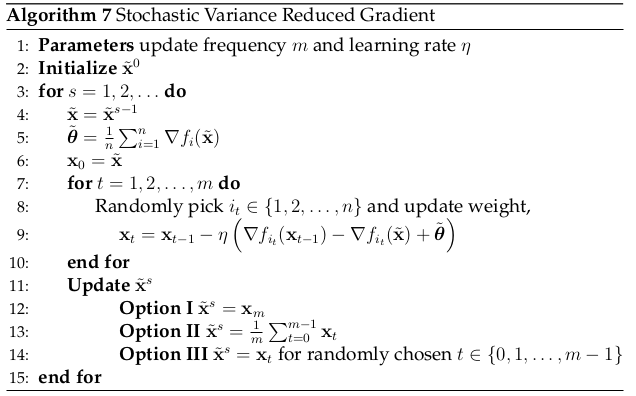
\includegraphics[scale=0.20]{ODS/images/SVRG.png}
\end{wrapfigure}
\textbf{SAGA}:The idea of SAGA is similar to SAG except that SAGA uses a different coefficient to keep the gradient estimator unbiased. SAGA works as follows: $\xx_{t+1} = \xx_t - \gamma\Big[(\nabla f_{i_t}(\xx_t) - \vv_{i_t}^{t-1})$ $  +\frac{1}{n}\sum_{i=1}^n{\vv_i^{t-1}} \Big]$. \\
\textbf{SVRG}: The idea of the algorithm is to use fixed reference point to build the variance-reduced gradient: $\vecg_t = \nabla f_{i_t}(\xx_t) - \nabla f_{i_t}(\Tilde{\xx}) + \nabla F(\Tilde{x})$, where the reference point $\Tilde{\xx}$ is only updated once a while. \\
\textbf{Convergence}: Assume $f_i(\xx)$ is convex and $L$-smooth and $F(\xx)= \frac{1}{n}\sum_{i=1}^n{f_i(\xx)}$ is $\mu$-strongly convex. Let $\xx^* = \argmin_{\xx}{F(\xx)}$, assume that $m$ is sufficiently large, and $\eta \leq \frac{1}{2L}$, so that $\rho = \frac{1}{\mu \eta (1 - 2L\eta) m} + \frac{2L \eta}{1 - 2L\eta} < 1$, then then we have geometric convergence in expectation for SVRG under Option II and III: $\E[F(\Tilde{\xx}^s) - F(\xx^*)] \leq \rho^s [F(\Tilde{\xx}^0) - F(\xx^*)]$. The trick is to prove the lemma: for any $\xx$ we have: $\frac{1}{n}\sum_{i=1}^n{\norm{\nabla f_i(\xx) - \nabla f_i(\xx^*)}_2^2} \leq 2L(F(\xx) - F(\xx^*))$. $\kappa_{\max} := \frac{L_{\max}}{\mu}$. \\
